\lecture{Material Requirements Planning}{18~-~02~-~2026}
%
%
\section{Introduzione}
Il \textbf{Material Requirements Planning} (MRP) è la metodologia standard per la gestione della domanda dipendente, ovvero la domanda di componenti, sottoassemblati e materie prime che è direttamente legata alla produzione di un prodotto finito.

Sviluppato da Joseph Orlicky presso \emph{IBM}, il sistema si è imposto a partire dal 1972 grazie alla ``MRP Crusade'' lanciata dall'APICS (\emph{American Production and Inventory Control Society}).

L'obiettivo fondamentale dell'MRP è garantire che i materiali siano disponibili nel momento esatto in cui sono richiesti, traslando temporalmente gli ordini di rifornimento.

%
\subsection{Composizione del sistema MRP}

%
\paragraph{Funzioni dell'MRP}
Il Material Requirements Planning si basa su 2 funzioni principali:
\begin{enumerate}
    \item \textbf{Derivare} la domanda dipendente per sottoassemblati, componenti e materie prime;
    \item \textbf{Traslare} temporalmente gli ordini di rifornimento in modo che i materiali siano disponibili nelle date in cui sono richiesti.
\end{enumerate}


%
\paragraph{5 Azioni dell'MRP}
Il processo di pianificazione segue una logica sequenziale rigorosa:
\begin{enumerate}
    \item \textbf{Netting}: Calcolo del fabbisogno netto (cosa mi serve davvero, sottraendo ciò che ho già);
    \item \textbf{Lot Sizing}: Raggruppamento del fabbisogno netto in lotti di produzione o acquisto economicamente o logisticamente validi;
    \item \textbf{Time Phasing} (Offsetting): Determinazione della data di rilascio dell'ordine, anticipando la data di consegna necessaria del valore del Lead Time;
    \item \textbf{BOM Explosion}: Calcolo del fabbisogno lordo dei componenti di livello inferiore basandosi sugli ordini pianificati del padre;
    \item \textbf{Iterate}: Ripetizione del processo per tutti i livelli della distinta base.
\end{enumerate}
%
\paragraph{I 3 componenti dell'MRP}
Il funzionamento dell'MRP si basa sull'interazione di tre input principali che alimentano il motore di calcolo:
\begin{enumerate}
    \item \textbf{Master Production Schedule} (MPS): Il piano principale di produzione che definisce cosa produrre (prodotti finiti), in quali quantità e quando;
    \item \textbf{Bill of Materials} (BOM): L'elenco strutturato che definisce la relazione padre-figlio tra il prodotto finito (end-item) e i suoi componenti (lower-level items);
    \item \textbf{Inventory Records}: Lo stato delle scorte, che include giacenze attuali, ordini già emessi e parametri di gestione (lead time, lot sizing).
\end{enumerate}

%
\subparagraph{Struttura dell'Inventory Record} Per ogni articolo, il sistema contiene le informazioni necessarie alla gestione della sua domanda dipendente.
Vedi figura \ref{fig:invrec}.
\begin{figure}
    \centering
    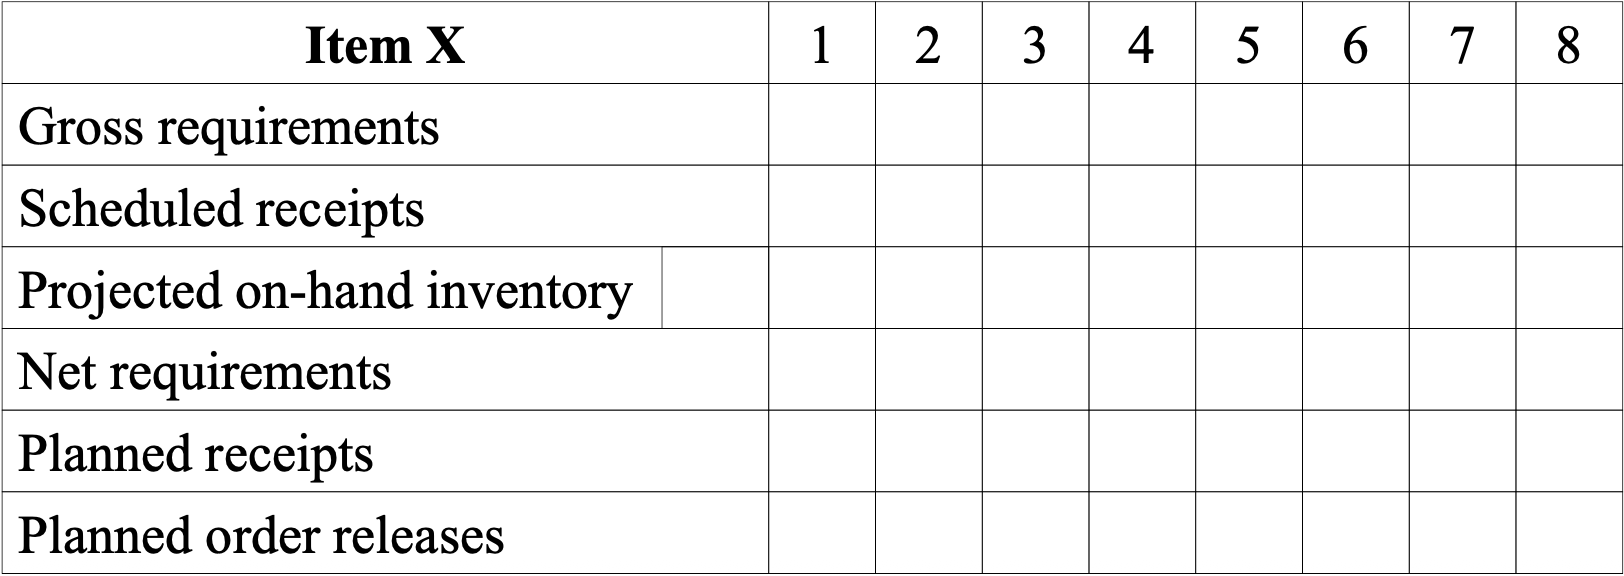
\includegraphics[width=0.7\linewidth]{assets/Screenshot 2026-02-18 at 10.01.35.png}
    \caption{Struttura dell'Inventory Record}\label{fig:invrec}
\end{figure}

L'inventory record ha queste voci fondamentali:
\begin{itemize}
    \item \textbf{Gross Requirements} (GR): Domanda totale derivata da tutti i piani di produzione dei livelli superiori;
    \item \textbf{Scheduled Receipts} (SR): Ordini già rilasciati ma non ancora completati nel momento in cui si pianifica l'attuale inventory record;
    \item \textbf{Projected On-Hand inventory} ($ \mathit{POH}(t) $): Quantità disponibile dell'articolo in ogni time bucket:
          \[
              I(t) = I(t-1) + \mathit{SR}(t) + \mathit{PR}(t) - \mathit{GR}(t)
          \]
    \item \textbf{Net Requirements} (NR): Domanda totale depurata del materiale in arrivo o disponibile a magazzino. Se $ t^{*} $ è il primo time bucket in cui $ \mathit{POH}(t) $ è negativo:
          \begin{flalign*}
               & N(t)           = 0 \quad \text{per} \quad t<t^{*},     &
               & N(t)           = -I(t) \quad \text{per} \quad t=t^{*}, &
               & N(t)           = G(t) \quad \text{per} \quad t>t^{*}   &   &
          \end{flalign*}

    \item \textbf{Planned Receipts} (PR): Consegne pianificate dell'articolo per mantenere il livello del $ \mathit{POH}(t) $ al di sopra del livello di sicurezza;
    \item \textbf{Planned Order Releases} (POR): Ordini di produzione/acquisto dell'articolo rilasciati affichè venga nella quantità e nella data prevista. La data di rilascio è la data di consegna prevista nel $ \mathit{PR}(t)-LT $ ($ LT = \text{Lead Time} $).
\end{itemize}

%
\subsubsection{Low-Level Code}
La BOM è organizzata a livelli: il prodotto finito è a Livello 0, i sottoassemblati diretti a Livello 1, e così via.

Quando un componente appare a più livelli diversi della distinta base (ad esempio, un bullone usato sia nel sottoassemblato base che nel prodotto finale), l'MRP lo elabora solo quando raggiunge il livello più basso in cui esso compare. L'\emph{LLC} è l'indice del livello più basso della BOM in cui compare il componente. Questo assicura che tutti i fabbisogni lordi (Gross Requirements) siano stati raccolti prima di procedere al calcolo del fabbisogno netto (Netting).

%
\section{Aggiornare l'MRP}
L'MRP non è statico: deve reagire a nuovi ordini, ritardi o modifiche tecniche. Esistono due approcci all'aggiornamento:
\begin{enumerate}
    \item \textbf{Regenerative MRP}: Ricalcola l'intero piano dall'inizio (MPS) esplodendo tutti i livelli. Elimina errori precedenti ma richiede elevate risorse di calcolo;
    \item \textbf{Net Change MRP}: Modifica solo le parti del piano coinvolte dal cambiamento. È più rapido ma tende ad accumulare errori, richiedendo rigenerazioni periodiche;
    \item \textbf{Top Down Planning}: Applica l'MRP tenendo conto dei dati modificati (MPS quantity e Scheduled receipts) ricalcolando il piano (può generare piani inammissibili, deve minimizzare i lead time, non riconosce piani MPS inammissibili);
    \item \textbf{Bottom Up Replanning}: Utilizza il Pegging e i Firm planned orders per guidare la ripianificazione (Pegging: collega i materiali agli ordini MPS; Firm planed orders producono materiali indipendentemente da ordini cliente e lead time).
\end{enumerate}

%
\subsection{Problema del nervosismo} L'MRP soffre di instabilità chiamata ``\emph{nervosismo}''. Piccole modifiche ai piani di alto livello (es. un leggero aumento della domanda nel MPS) possono causare cambiamenti drastici e sproporzionati nei piani dei livelli inferiori.
\begin{example}
    Un piccolo aumento di richiesta può costringere ad anticipare un intero lotto di produzione a causa delle regole di lot-sizing rigide (come il Period Order Quantity o Fixed Order Quantity), alterando completamente le date di rilascio ordini per i componenti.
\end{example}

%
\subsubsection{Strumenti di stabilizzazione e controllo}
%
\paragraph{Pegging} Funzionalità che associa i fabbisogni lordi agli ordini rilasciati al livello superiore della BOM (single pegging) o all'ordine cliente (full pegging).
%
\paragraph{Firm Planned Orders} Ordini che il sistema MRP non può modificare autonomamente al variare delle condizioni. Sono utilizzati per stabilizzare il sistema.

%
\section{Limiti dell'MRP}
Come tutto, anche l'MRP ha delle limitazioni:
\begin{itemize}
    \item \textbf{Integrità dei dati}: deve essere rispettata al 99\%
    \item \textbf{Lead time fissi}: Devono essere noti a priori e sono costanti nel tempo, indipendentemente dalla quantità da produrre e dallo stato del sistema;
    \item \textbf{Localizzazione fisica dei materiali}: Avere disponibilità di materiali in un magazzino a chilometri di distanza non serve;
    \item \textbf{Variabilità BOM}: Le modifiche della BOM devono essere registrate e conservate nel tempo;
    \item \textbf{Capacità produttiva}: Non viene considerata e quindi si hanno piani di produzione non ammissibili;
    \item \textbf{Contabilità}: Non vi è collegamento con gli aspetti contabili dell'azienda;
    \item \textbf{Previsioni}: non esiste un sistema di previsione della domanda.
\end{itemize}

%
\section{MRP II}
L'MRP II nasce per superare i limiti dell'MRP semplice, integrando la pianificazione delle risorse e la verifica della capacità.

Gerarchia di Pianificazione MRP II:
\begin{enumerate}
    \item \textbf{Lungo Termine}: Aggregate Production Planning;
    \item \textbf{Medio Termine}: MPS validato tramite RCCP (Rough-Cut Capacity Planning). L'RCCP verifica la fattibilità del piano principale sulle risorse critiche prima di lanciare l'MRP;
    \item \textbf{Breve Termine} (Esecuzione):
          \begin{itemize}
              \item \textbf{CRP} (Capacity Requirements Planning): Più dettagliato dell'RCCP, usa i dati dei cicli di lavoro (routing) per identificare sovraccarichi sui centri di lavoro;
              \item \textbf{PAC} (Production Activity Control): Monitora l'esecuzione, gestisce le priorità e controlla l'input/output effettivo rispetto al pianificato.
          \end{itemize}
\end{enumerate}

%
\section{MRP Fundamental Flaw}

\begin{quote}[1975]{Orlicky}
    An MRP system is capacity-insensitive, and properly so, as its function is to determine what materials and components will be needed and when, in order to execute a given master production schedule. There can be only one correct answer to that, and it cannot therefore vary depending on what capacity does or does not exist.
\end{quote}